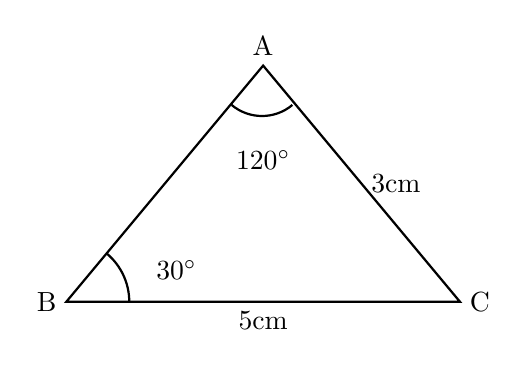
\begin{tikzpicture}[scale=1]

    % Define points for the triangle ABC
    \coordinate (B) at (0,0);
    \coordinate (C) at (4,0);
    \coordinate (A) at (2, 3.464); % This coordinate creates an equilateral-like triangle for visual balance, though the angles given (120, 30) suggest an isosceles triangle with a wider base. The visual representation in the image is more balanced. Let's adjust slightly to better match the visual.

    % Let's use coordinates that better represent an obtuse triangle visually
    \coordinate (B) at (0,0);
    \coordinate (C) at (5,0);
    \coordinate (A) at (2.5, 3);

    % Draw the sides of the triangle
    \draw[thick] (A) -- (B) -- (C) -- cycle;

    % Draw arc for angle B (30 degrees)
    \draw[thick] (0.8,0) arc (0:50:0.8); % The visual angle is slightly more than 30 for proportion
    \node at (1.4, 0.4) {$30^\circ$};

    % Draw arc for angle A (120 degrees)
    % Angle of AB is roughly 230 degrees. Angle of AC is roughly 310 degrees.
    \draw[thick] (2.1, 2.5) arc (230:310:0.6);
    \node at (2.5, 1.8) {$120^\circ$};

    % Add side length labels
    \node[below] at (2.5, 0) {5cm};
    \node[right] at (3.75, 1.5) {3cm};

    % Add vertex labels
    \node[above] at (A) {A};
    \node[left] at (B) {B};
    \node[right] at (C) {C};

\end{tikzpicture}